\begin{enumerate}[\large\bfseries 1.]

%-------------------- 1.
\item  
\begin{enumerate}[\bfseries a)]
    
    %----------a)
    \item \textbf{Análisis del problema.}\\\\
	Para poder hallar establecemos primero el ancho del pincel, luego el color de fondo, y a través de un vector definiremos los colores a dibujar.\\
	Ahora utilizaremos un loop for para iterar 120 veces. Cabe mencionar que para cambiar el color de brecha vamos a sincronizarlo con el vector creado.\\
	Para la longitud de las lineas vamos a aplicar la siguiente formula.
	$$i+(i*2))$$\\

    %----------d)
    \item \textbf{Código fuente.}\\ 
	
	\lstinputlisting[language=Python]{python/tarea5/ej1.py}
	\vspace{10cm}
    
    %----------e)
    \item \textbf{Prueba de la ejecución del programa}.\\
	\begin{center}
	    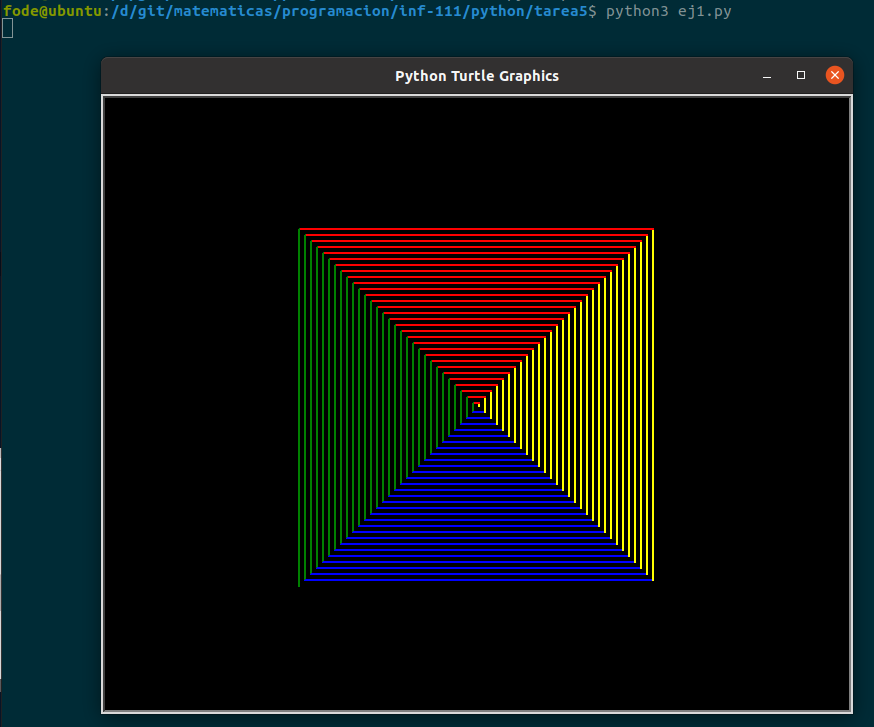
\includegraphics[scale=.5]{imagenes/tarea5/ej1.png}
	\end{center}

\end{enumerate}

\newpage

%--------------------2.
\item 
\begin{enumerate}[\bfseries a)]
    
    %----------a)
    \item \textbf{Análisis del problema.}\\\\

    %----------b)
    \item \textbf{Diagrama de flujo.}\\
	\begin{center}
	    %\includegraphics[scale=.37]{imagenes/tarea5}
	\end{center}

    %----------c)
    \item \textbf{Prueba de escritorio.}\\
	\begin{center}
	    \begin{tabular}{c|c}
		Dibujo&Print\\
		\hline
		t&Dibujar un triangulo\\
		\hline
		r&Dibujar un rectángulo\\
		\hline
		c&Dibujar un Circulo\\
	    \end{tabular}
	\end{center}
	\vspace{4cm}
    
    %----------d)
    \item \textbf{Código fuente.}\\ 
	
	%\lstinputlisting[language=Python]{python/tarea5}
	\vspace{3cm}
    
    %----------e)
    \item \textbf{Prueba de la ejecución del programa}.\\
	\begin{center}
	    %\includegraphics[scale=.5]{imagenes/tarea5}
	\end{center}

\end{enumerate}

\newpage

\end{enumerate}
